% ======================================================================
% figures.tex  --  all figures for the GenoLeWM paper.
% Self-contained: requires tikz, pgfplots, xcolor (loaded in main preamble).
% Color + style definitions are guarded so this file also compiles standalone.
% ======================================================================
\providecommand{\genocolor}{}\definecolor{genocolor}{HTML}{2F6F9F}
\providecommand{\carboncolor}{}\definecolor{carboncolor}{HTML}{C24A3B}
\providecommand{\baselinecolor}{}\definecolor{baselinecolor}{HTML}{8A8A8A}
\definecolor{statefill}{HTML}{EAF1F7}
\definecolor{actfill}{HTML}{FBE9E6}

% ----------------------------------------------------------------------
% Figure 1: system architecture / latent-edit pipeline
% ----------------------------------------------------------------------
\newcommand{\figArchitecture}{%
\begin{figure}[t]
  \centering
  \resizebox{\linewidth}{!}{%
  \begin{tikzpicture}[
    font=\small,
    box/.style={draw,rounded corners=2pt,minimum height=8mm,inner sep=4pt,align=center},
    frozen/.style={box,draw=genocolor,fill=statefill,very thick},
    train/.style={box,draw=carboncolor,fill=actfill,very thick},
    io/.style={align=center,font=\footnotesize},
    lat/.style={circle,draw,minimum size=8mm,inner sep=1pt,font=\footnotesize,align=center},
    arr/.style={-{Stealth[length=2.2mm]},thick},
  ]
    \node[io] (edit) {edit action $a$\\[-1pt]\scriptsize(pos, type, ref, alt)};
    \node[io,below=10mm of edit] (wref) {reference window\\[-1pt]$w_{\mathrm{ref}}$ ($4{,}096$\,bp released)};
    \node[io,below=12mm of wref] (walt) {edited window\\[-1pt]$w_{\mathrm{alt}}$};

    \node[train,right=12mm of edit] (aenc) {action\\encoder};
    \node[frozen,right=12mm of wref] (enc1) {Carbon-500M\\encoder \textbf{(frozen)}};
    \node[frozen,right=12mm of walt] (enc2) {Carbon-500M\\encoder \textbf{(frozen)}};

    \node[lat,right=10mm of aenc] (aemb) {$a_{\mathrm{emb}}$};
    \node[lat,right=10mm of enc1] (st) {$s_t$ raw\\[-2pt]\scriptsize global};
    \node[lat,right=10mm of enc2] (stp1) {$s_{t+1}$ raw\\[-2pt]\scriptsize centered};

    \node[train,right=16mm of st,minimum height=13mm] (pred) {cross-attention\\predictor $g$};
    \node[lat,right=12mm of pred] (shat) {$\hat s_{t+1}$ unit};
    \node[box,draw=black!55,right=10mm of shat] (loss) {$\mathcal{L}_{\mathrm{pred}}$};
    \draw[arr] (edit) -- (aenc);
    \draw[arr] (wref) -- (enc1);
    \draw[arr] (walt) -- (enc2);
    \draw[arr] (aenc) -- (aemb);
    \draw[arr] (enc1) -- (st);
    \draw[arr] (enc2) -- (stp1);
    \draw[arr] (aemb) -| ([xshift=-4mm]pred.north) -- (pred.north);
    \draw[arr] (st) -- (pred);
    \draw[arr] (pred) -- (shat);
    \draw[arr] (shat) -- (loss);
    \draw[arr] (stp1) -| (loss.south);
    \begin{scope}[on background layer]
      \node[fit=(enc1)(enc2)(wref)(walt),draw=genocolor,dashed,rounded corners,inner sep=6pt,
        label={[genocolor,font=\footnotesize]above:frozen state encoder (paid once per window)}] {};
    \end{scope}
  \end{tikzpicture}}
  \caption{\textbf{Released v0.2.1-r1 computation, exposing the state-contract violation.}
  A frozen Carbon-500M DNA encoder maps a reference window $w_{\mathrm{ref}}$ to a state
  $s_t\in\mathbb{R}^{1024}$; a small trainable action encoder maps an explicit edit
  $a=(\text{pos},\text{type},\text{ref},\text{alt})$ to $a_{\mathrm{emb}}$; and a cross-attention
  predictor $g$ returns $\hat s_{t+1}=g(s_t,a_{\mathrm{emb}})$. Although \texttt{normalize: true} was
  configured, released source and target encoder states were raw (rollout mean norms $29$--$34$), while
  the predictor output was unit norm. Training sources used global pooling while targets used edit-centered
  pooling; every nominal edit center also omitted the leading \texttt{<dna>} token and was shifted one hidden token left.
  Rollout changed the source coordinate again. The frozen target-only KL had no gradient and no LoRA was present.
  The diagram documents implementation flow, not validated world-model capability.}
  \label{fig:architecture}
\end{figure}}

% ----------------------------------------------------------------------
% Figure 2: VEP results vs Carbon zero-shot
% ----------------------------------------------------------------------
\newcommand{\figVEP}{%
\begin{figure}[t]
  \centering
  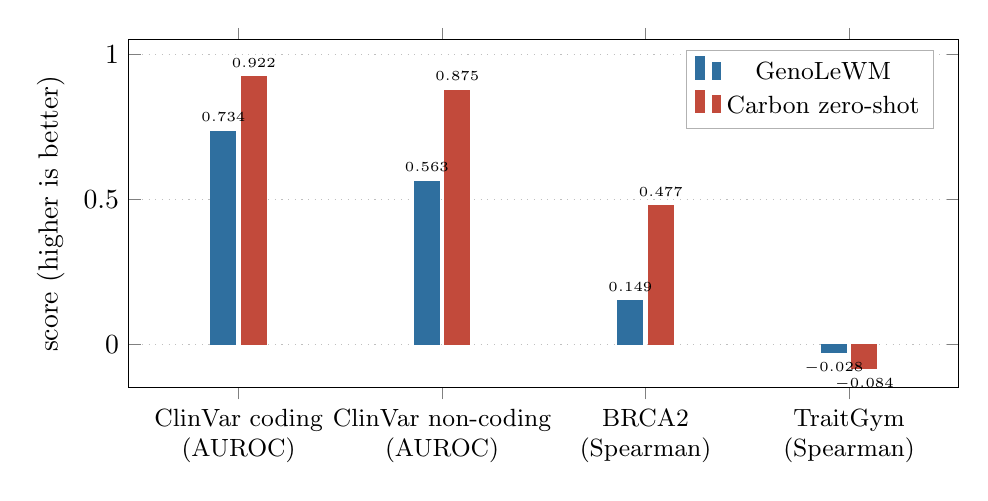
\begin{tikzpicture}
  \begin{axis}[
    width=\linewidth, height=6cm, ybar, bar width=9pt,
    ymin=-0.15, ymax=1.05,
    ylabel={score (higher is better)},
    symbolic x coords={ClinVar coding\\(AUROC),ClinVar non-coding\\(AUROC),BRCA2\\(Spearman),TraitGym\\(Spearman)},
    xtick=data, xticklabel style={align=center,font=\small},
    legend pos=north east, legend style={font=\small,draw=black!30},
    enlarge x limits=0.18, ymajorgrids, grid style=dotted,
    nodes near coords, every node near coord/.append style={font=\tiny,/pgf/number format/.cd,fixed,precision=3},
  ]
  \addplot[fill=genocolor,draw=genocolor] coordinates {
    ({ClinVar coding\\(AUROC)},0.734375)
    ({ClinVar non-coding\\(AUROC)},0.5625)
    ({BRCA2\\(Spearman)},0.149194)
    ({TraitGym\\(Spearman)},-0.0279645)};
  \addplot[fill=carboncolor,draw=carboncolor] coordinates {
    ({ClinVar coding\\(AUROC)},0.921875)
    ({ClinVar non-coding\\(AUROC)},0.875)
    ({BRCA2\\(Spearman)},0.476907)
    ({TraitGym\\(Spearman)},-0.0838935)};
  \legend{GenoLeWM, Carbon zero-shot}
  \end{axis}
  \end{tikzpicture}
  \caption{\textbf{Historical v0.2.1 VEP rows; withdrawn as a method comparison.} Carbon values are
  recovered as GenoLeWM~$-$~$\Delta$. The GenoLeWM ranking score came from an $L_2$ residual between
  unit-norm predictions and raw target states, so bar differences do not establish better or worse
  performance for the intended normalized-state method. The small slices add a separate power
  limitation; see \S\ref{sec:limitations}.}
  \label{fig:vep}
\end{figure}}

% ----------------------------------------------------------------------
% Figure 3: rollout fidelity vs source-state baseline (the baseline trap)
% ----------------------------------------------------------------------
\newcommand{\figRollout}{%
\begin{figure}[t]
  \centering
  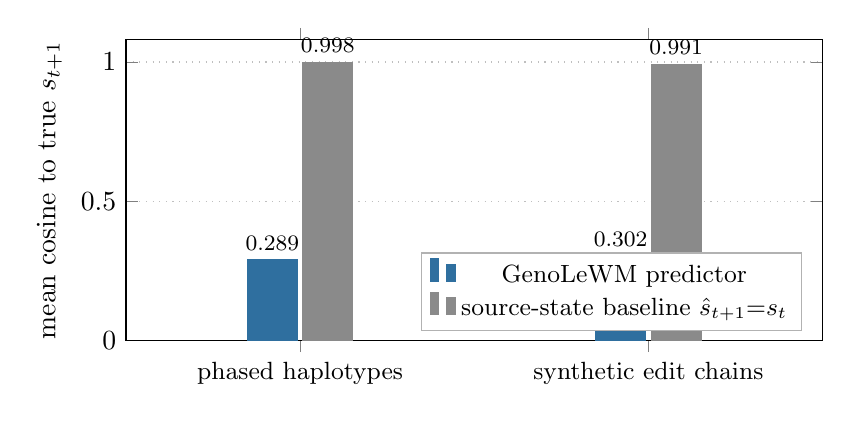
\begin{tikzpicture}
  \begin{axis}[
    width=0.86\linewidth, height=5.4cm, ybar, bar width=18pt,
    ymin=0, ymax=1.08,
    ylabel={mean cosine to true $s_{t+1}$},
    symbolic x coords={phased haplotypes,synthetic edit chains},
    xtick=data, xticklabel style={font=\small},
    legend pos=south east, legend style={font=\small,draw=black!30},
    enlarge x limits=0.5, ymajorgrids, grid style=dotted,
    nodes near coords, every node near coord/.append style={font=\footnotesize,/pgf/number format/.cd,fixed,precision=3},
  ]
  \addplot[fill=genocolor,draw=genocolor] coordinates {(phased haplotypes,0.288861) (synthetic edit chains,0.301608)};
  \addplot[fill=baselinecolor,draw=baselinecolor] coordinates {(phased haplotypes,0.997831) (synthetic edit chains,0.991239)};
  \legend{GenoLeWM predictor, source-state baseline $\hat s_{t+1}{=}s_t$}
  \end{axis}
  \end{tikzpicture}
  \caption{\textbf{Historical rollout cosine; mechanism withdrawn.} Prediction-to-target cosine is
  $\approx0.29$--$0.30$ and raw-source-to-target cosine is $\approx0.99$. Cosine is scale-invariant, so
  these values remain historical measurements, but the predictor was trained with a mixed-scale $L_2$
  term, mixed pooling coordinates, a one-hidden-token centering offset, and rollout differs from the training distribution. The gap therefore does not establish a
  latent-residual trap, action-conditioning failure, or any other mechanism (\S\ref{sec:discussion}).}
  \label{fig:rollout}
\end{figure}}

% ----------------------------------------------------------------------
% Figure 4: AR rollout speedup vs target
% ----------------------------------------------------------------------
\newcommand{\figARspeed}{%
\begin{figure}[t]
  \centering
  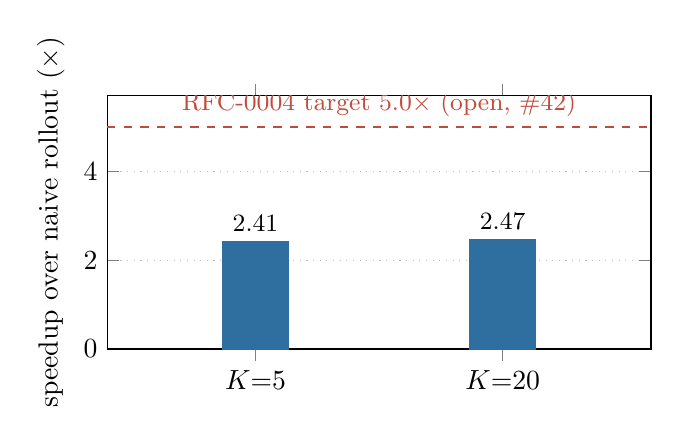
\begin{tikzpicture}
  \begin{axis}[
    width=0.7\linewidth, height=4.8cm, ybar, bar width=24pt,
    ymin=0, ymax=5.7,
    ylabel={speedup over naive rollout ($\times$)},
    symbolic x coords={$K{=}5$,$K{=}20$},
    xtick=data, enlarge x limits=0.6, ymajorgrids, grid style=dotted,
    nodes near coords, every node near coord/.append style={font=\small,/pgf/number format/.cd,fixed,precision=2},
  ]
  \addplot[fill=genocolor,draw=genocolor] coordinates {({$K{=}5$},2.41386) ({$K{=}20$},2.47322)};
  \draw[carboncolor,thick,dashed]
    ({rel axis cs:0,0}|-{axis cs:$K{=}5$,5.0}) -- ({rel axis cs:1,0}|-{axis cs:$K{=}20$,5.0})
    node[pos=0.5,above,font=\small,carboncolor]{RFC-0004 target $5.0\times$ (open, \#42)};
  \end{axis}
  \end{tikzpicture}
  \caption{\textbf{Historical KV-cache micro-benchmark.} Cached \texttt{ARPredictor} rollout is
  $2.41\times$ ($K{=}5$) and $2.47\times$ ($K{=}20$) faster than naive repeated one-step prediction.
  The gain is real but short of the $5\times$ target at $K{=}20$, which remains open and was explicitly rescoped.
  Measured on synthetic tensors with batch $8$, $d_{\mathrm{state}}{=}1024$, $d_{\mathrm{action}}{=}64$, CUDA, and bf16 on H200. The benchmark-specific predictor ($d_{\mathrm{hidden}}{=}1024$, $6+1$ blocks, FFN $4096$) is not the exact released checkpoint.}
  \label{fig:arspeed}
\end{figure}}

% ----------------------------------------------------------------------
% Figure: efficiency three-regime latency decomposition
% ----------------------------------------------------------------------
\newcommand{\figEfficiency}{%
\begin{figure}[t]
  \centering
  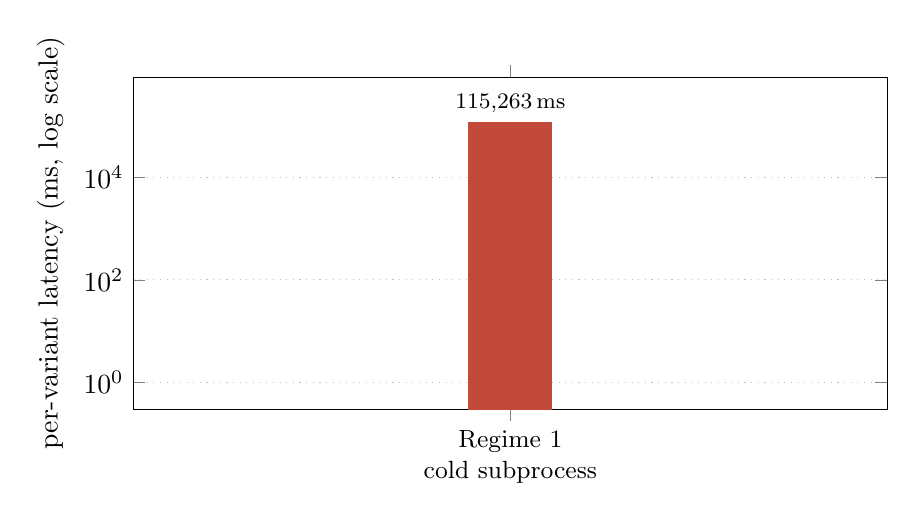
\begin{tikzpicture}
  \begin{semilogyaxis}[
    width=0.92\linewidth, height=5.8cm, ybar, bar width=30pt,
    ymin=0.3, ymax=900000, ymode=log, log origin=infty,
    ylabel={per-variant latency (ms, log scale)},
    symbolic x coords={Regime 1\\cold subprocess,Regime 2\\warm cache,Regime 3\\latent rollout},
    xtick=data, xticklabel style={align=center,font=\small},
    enlarge x limits=0.28, ymajorgrids, grid style=dotted,
    point meta=explicit symbolic,
    nodes near coords, every node near coord/.append style={font=\footnotesize,anchor=south},
  ]
  \addplot[fill=carboncolor,draw=carboncolor] coordinates {
    ({Regime 1\\cold subprocess},115262.94) [115{,}263\,ms]};
  \end{semilogyaxis}
  \end{tikzpicture}
  \caption{\textbf{Historical cold-process timing.} Only \emph{Regime 1}, a cold \texttt{geno-lewm-score} subprocess (interpreter start,
  ${\sim}1$\,GiB Carbon load, two Carbon forward passes), is measured, at $115{,}262.94$\,ms. The
  release did not profile component timing, so this total cannot be apportioned between loading and compute. The
  ``pay-Carbon-once'' thesis applies to \emph{Regime 2} (warm reference cache: one Carbon call on the
  edited window, in-process) and \emph{Regime 3} (latent-only rollout/planning: zero further Carbon
  calls), both \emph{unmeasured} on this checkpoint and therefore shown without bars. Because corresponding model quality is invalidated, this figure
  supports neither a deployment claim nor an efficiency--quality comparison.}
  \label{fig:efficiency}
\end{figure}}
